\documentclass[11pt,letterpaper]{article}
\usepackage[utf8]{inputenc}
\usepackage[T1]{fontenc}
\usepackage[provide=*,english]{babel}
\usepackage{lmodern}
\usepackage{amsmath,amssymb,amsfonts}
\usepackage[margin=2.5cm]{geometry}
\usepackage{fancyhdr}
\usepackage{enumitem}
\usepackage[most]{tcolorbox}
\usepackage{xcolor}
\usepackage{tikz}
\usetikzlibrary{arrows.meta,angles,quotes,calc,babel}
\usepackage{placeins}
\usepackage{graphicx}
\usepackage{microtype}
\usepackage{needspace}
% ============ PALETTE: BLACK, ORANGE, AND CREAM ============
\definecolor{blackmain}{HTML}{1A1A1A}
\definecolor{orangeacc}{HTML}{E65C00}
\definecolor{creambg}{HTML}{FBF8F1}
\definecolor{orangebg}{HTML}{FFF4EB}
\definecolor{graymuted}{HTML}{7A746E}
\definecolor{pureblack}{HTML}{0D0D0D}
% ============ HEADERS AND FOOTERS ============
\setlength{\headheight}{24pt}
\pagestyle{fancy}
\fancyhf{}
\fancyhead[L]{\textcolor{blackmain}{\textbf{\small Mathematical Methods I}}}
\fancyhead[R]{\textcolor{orangeacc}{\textbf{\small Differential 1-forms}}}
\fancyfoot[C]{\textcolor{graymuted}{\thepage}}
\renewcommand{\headrulewidth}{0.8pt}
\renewcommand{\headrule}{\hbox to\headwidth{\color{orangeacc}\leaders\hrule height \headrulewidth\hfill}}
\setlist[itemize]{label={\small\textcolor{orangeacc}{$\blacksquare$}},leftmargin=1.6em}
\setlist[enumerate]{label={\textcolor{orangeacc}{\arabic*.}},leftmargin=1.8em}
% ============ TITLES ============
\newcommand{\manualsection}[1]{%
  \Needspace{16\baselineskip}%
  \vspace{0.35cm}
  \par\noindent{\Large\bfseries\color{blackmain} #1}\par\nobreak
  \noindent{\color{orangeacc}\rule{\linewidth}{1.4pt}}\par\nobreak
  \vspace{0.15cm}
}
\newcommand{\manualsubsection}[1]{%
  \par\vspace{0.2cm}\noindent{\bfseries\color{orangeacc} #1}\par\nobreak
  \vspace{0.12cm}
}
% ============ CONTENT BOXES ============
\newtcolorbox{infobox}[2][orangeacc]{
  enhanced,
  colback=creambg,colframe=#1!90!black,
  boxrule=1pt,arc=2mm,
  left=9pt,right=9pt,top=5pt,bottom=5pt,
  before skip=7pt,after skip=7pt,
  before upper={\textbf{\color{#1!95!black}\large #2}\par\nobreak
    {\color{#1!50}\rule{\linewidth}{0.6pt}}\par\nobreak\smallskip}
}
\newtcolorbox{examplebox}[1]{
  enhanced,
  colback=orangebg,colframe=orangeacc!85!black,
  boxrule=1pt,arc=2mm,
  left=9pt,right=9pt,top=5pt,bottom=5pt,
  before skip=7pt,after skip=7pt,
  before upper={\textbf{\color{orangeacc!95!black}\large #1}\par\nobreak
    {\color{orangeacc!40}\rule{\linewidth}{0.6pt}}\par\nobreak\smallskip}
}
\newtcolorbox{theorembox}[1]{
  enhanced,
  colback=creambg!70!white,colframe=pureblack,
  boxrule=1.1pt,arc=2mm,
  left=9pt,right=9pt,top=5pt,bottom=5pt,
  before skip=7pt,after skip=7pt,
  before upper={\textbf{\color{pureblack}\large #1}\par\nobreak
    {\color{orangeacc}\rule{\linewidth}{0.8pt}}\par\nobreak\smallskip}
}
\newcommand{\term}[1]{\textbf{\color{orangeacc}#1}}
\newcommand{\termb}[1]{\textbf{\color{blackmain}#1}}
\renewcommand{\familydefault}{\rmdefault}
\linespread{1.05}
\tikzset{every node/.append style={font=\rmfamily}}
\begin{document}
\setlength{\abovedisplayskip}{6pt}
\setlength{\belowdisplayskip}{6pt}
\setlength{\abovedisplayshortskip}{4pt}
\setlength{\belowdisplayshortskip}{4pt}
\setlength{\textfloatsep}{10pt}
\setlength{\intextsep}{8pt}
\setlength{\jot}{2pt}
\color{blackmain}
\begin{center}
{\LARGE\textbf{Mathematical Methods I}}\\[0.2cm]
{\Large\textcolor{orangeacc}{\textbf{Differential 1-forms}}}\\[0.4cm]
{\large\textcolor{graymuted}{Gabriel Velázquez}}\\[0.25cm]
\end{center}
\manualsection{1. Covectors and 1-forms}
A tangent vector describes a direction and a magnitude at a point. A 1-form evaluates that vector and produces a real number in a linear way.
\begin{infobox}[orangeacc]{Definition 1.1 (Covector and covector field)}
Let $\Omega\subseteq\mathbb{R}^n$ be open. A \term{covector} at $p\in\Omega$ is a linear map
\[
\omega_p:T_p\Omega\longrightarrow\mathbb{R}.
\]
The set of these functionals is the \term{cotangent space}
$T_p^*\Omega=(T_p\Omega)^*$, the dual of the tangent space.
A \term{differential 1-form} $\omega$ assigns a covector $\omega_p$ to each point $p$, with smooth coefficient functions in the case of a smooth form.
\end{infobox}
Linearity refers to vectors based at the same point: for $u_p,v_p\in T_p\Omega$ and $a,b\in\mathbb{R}$,
\[
\omega_p(au_p+bv_p)=a\omega_p(u_p)+b\omega_p(v_p).
\]
\begin{theorembox}{Operations with 1-forms}
For 1-forms $\phi,\psi$ and a scalar function $f$, define
\begin{align*}
(\phi+\psi)_p(v_p)&=\phi_p(v_p)+\psi_p(v_p),\\
(f\phi)_p(v_p)&=f(p)\,\phi_p(v_p).
\end{align*}
The factor $f$ is evaluated at the base point of the vector; it is not differentiated.
\end{theorembox}
\manualsubsection{Evaluation on a vector field}
If $X$ is a vector field, $\omega(X)$ is the scalar function
\[
\bigl(\omega(X)\bigr)(p)=\omega_p(X(p)).
\]
In particular, $\omega_p(v_p)$ is a number, whereas $\omega(X)$ is a function of $p$.
\begin{theorembox}{Linearity over functions}
For vector fields $X,Y$ and scalar functions $f,g$,
\[
\omega(fX+gY)=f\,\omega(X)+g\,\omega(Y).
\]
Thus, a 1-form transforms vector fields into functions by pointwise evaluation.
\end{theorembox}
\newpage
\manualsection{2. Coordinate differentials and the dual basis}
Let $x^1,\ldots,x^n$ be the Cartesian coordinate functions. We write
\[
U_j=\partial_j=\frac{\partial}{\partial x^j},
\qquad v_p=\sum_{j=1}^n v^j\,\partial_j\big|_p.
\]
The superscripts in $x^i$ and $v^i$ are indices, not powers.
\begin{infobox}[orangeacc]{Definition 2.1 (Differential of a function)}
For a differentiable function $f:\Omega\to\mathbb{R}$, its differential at $p$ is
\[
(df)_p(v_p)=v_p[f].
\]
The differentiability of $f$ guarantees that this expression is linear in $v_p$. If $f$ is smooth, $df$ is a smooth 1-form. Applied to $f=x^i$,
\[
(dx^i)_p(v_p)=v_p[x^i]=v^i.
\]
The coordinate 1-form $dx^i$ selects the $i$th component of the vector.
\end{infobox}
\begin{theorembox}{Proposition 2.2 (Duality of the bases)}
At each point, $\{(dx^1)_p,\ldots,(dx^n)_p\}$ is the dual basis of $\{\partial_1|_p,\ldots,\partial_n|_p\}$. Indeed,
\[
(dx^i)_p(\partial_j|_p)
=\partial_j|_p[x^i]
=\frac{\partial x^i}{\partial x^j}(p)
=\delta^i_j,
\qquad
\delta^i_j=\begin{cases}1,&i=j,\\0,&i\ne j.\end{cases}
\]
As an identity between functions, we write $dx^i(U_j)=\delta^i_j$.
\end{theorembox}
In Cartesian coordinates, the value $dx^i(v_p)=v^i$ does not explicitly depend on $p$ when the vector components are fixed.
\begin{figure}[htbp]
\centering
\begin{tikzpicture}[>=Stealth,scale=.9]
\draw[->,graymuted] (-.3,0)--(4.6,0) node[right] {$x$};
\draw[->,graymuted] (0,-.3)--(0,3.1) node[above] {$y$};
\coordinate (P) at (.7,.6); \coordinate (Q) at (3.7,2.6);
\draw[dashed,graymuted] (Q)--(3.7,.6);
\draw[dashed,graymuted] (P)--(.7,2.6)--(Q);
\draw[->,orangeacc,very thick] (P)--(Q) node[midway,above left] {$v_p$};
\draw[->,blackmain,thick] (P)--(3.7,.6) node[midway,below] {$v^x=dx(v_p)$};
\draw[->,blackmain,thick] (3.7,.6)--(Q) node[midway,right] {$v^y=dy(v_p)$};
\fill (P) circle (2pt) node[below left] {$p$};
\end{tikzpicture}
\caption{The forms $dx$ and $dy$ return the components of the vector based at $p$. The horizontal and vertical arrows represent vector components, not the 1-forms themselves.}
\end{figure}
\FloatBarrier
\newpage
\manualsection{3. Expression and evaluation of a 1-form}
\begin{theorembox}{Proposition 3.1 (Coordinate expression)}
Every 1-form can be uniquely expressed as
\[
\omega=\sum_{i=1}^n a_i\,dx^i,
\]
where the $a_i$ are scalar functions. Its coefficients are recovered by evaluating it on the tangent basis:
\[
a_i=\omega(U_i).
\]
\end{theorembox}
\manualsubsection{Proof and evaluation formula}
At a point $p$, let $v_p=\sum_jv^j\partial_j|_p$. By linearity and duality,
\begin{align*}
\omega_p(v_p)
&=\left(\sum_i a_i(p)(dx^i)_p\right)
  \left(\sum_j v^j\partial_j|_p\right)\\
&=\sum_i\sum_j a_i(p)v^j\,(dx^i)_p(\partial_j|_p)\\
&=\sum_i\sum_j a_i(p)v^j\delta^i_j
=\sum_i a_i(p)v^i.
\end{align*}
In particular,
\[
\omega(U_j)=\sum_i a_i\,dx^i(U_j)=\sum_i a_i\delta^i_j=a_j.
\]
Conversely, defining $a_i=\omega(U_i)$, the form $\sum_i a_i dx^i$ agrees with $\omega$ on every basis vector and, by linearity, on every vector. This proves the existence and uniqueness of the expression.
\begin{infobox}[orangeacc]{Evaluation on a vector field}
If $X=\sum_i X^i\partial_i$, then
\[
\boxed{\omega(X)=\sum_i a_iX^i.}
\]
Both sides are functions; evaluation at $p$ gives $\omega_p(X(p))$.
\end{infobox}
\begin{examplebox}{Example 3.2 (A function and its value at a point)}
In $\mathbb{R}^2$, let $\omega=y\,dx+2x\,dy$ and $X=x\partial_x-\partial_y$. Then
\[
\omega(X)=xy-2x.
\]
For $p=(1,3)$, $\omega_p=3(dx)_p+2(dy)_p$ and $X(p)=(1,-1)_p$, so $\omega_p(X(p))=3-2=1$.
Moreover, $\omega(\partial_x)=y$ and $\omega(\partial_y)=2x$ recover the coefficients.
\end{examplebox}
\newpage
\manualsection{4. The differential $df$ and exact forms}
\begin{theorembox}{Theorem 4.1 (Coordinate expression of the differential)}
For a differentiable function $f:\Omega\to\mathbb{R}$,
\[
\boxed{df=\sum_{i=1}^n\frac{\partial f}{\partial x^i}\,dx^i.}
\]
A 1-form that can be written as $df$ throughout its domain is called \term{exact}. The function $f$ is a potential for that form.
\end{theorembox}
\manualsubsection{Proof by evaluation}
For any $v_p=\sum_jv^j\partial_j|_p$, the definition of the differential gives
\[
(df)_p(v_p)=v_p[f]=\sum_i v^i\frac{\partial f}{\partial x^i}(p).
\]
On the other hand, using duality,
\begin{align*}
\left(\sum_i\frac{\partial f}{\partial x^i}(p)(dx^i)_p\right)(v_p)
&=\sum_i\sum_j\frac{\partial f}{\partial x^i}(p)v^j\delta^i_j\\
&=\sum_i\frac{\partial f}{\partial x^i}(p)v^i.
\end{align*}
The two forms agree on all tangent vectors and are therefore equal. Equivalently, their coefficients are obtained as
\[
df(U_i)=U_i[f]=\frac{\partial f}{\partial x^i}.
\]
\begin{examplebox}{Example 4.2 (Computing $df$)}
If $f(x,y,z)=x^2y+z^2$, then
\[
df=2xy\,dx+x^2\,dy+2z\,dz.
\]
For $p=(1,2,-1)$ and $v_p=(2,-1,3)_p$,
\[
(df)_p(v_p)=4(2)+1(-1)-2(3)=1.
\]
This gives the directional derivative of $f$ along the vector $v_p$.
\end{examplebox}
\manualsubsection{Differential, vector field, and curve}
For any vector field $X$, $df(X)=X[f]$. If $\alpha$ is a differentiable curve contained in $\Omega$, the chain rule states that
\[
(df)_{\alpha(t)}\bigl(\alpha'(t)\bigr)
=\frac{d}{dt}\bigl(f(\alpha(t))\bigr).
\]
Evaluating $df$ on the velocity measures how $f$ changes along the curve.
\newpage
\manualsection{5. The operator $d$: products and compositions}
The operator $d$ transforms a scalar function $f$ into the 1-form $df$. The usual differentiation rules thus become equalities between 1-forms. We assume that the functions are differentiable on their domains.
\begin{theorembox}{Proposition 5.1 (Linearity and the product rule)}
For $f,g:\Omega\to\mathbb{R}$ and constants $a,b\in\mathbb{R}$,
\[
d(af+bg)=a\,df+b\,dg,\qquad d(c)=0\quad(c\text{ constant}).
\]
The \term{Leibniz rule} states that
\[
\boxed{d(fg)=f\,dg+g\,df.}
\]
The factors $f$ and $g$ multiply 1-forms. At a point $p$, this equality means
\[
\bigl(d(fg)\bigr)_p=f(p)(dg)_p+g(p)(df)_p.
\]
\end{theorembox}
\manualsubsection{Why the product rule holds}
For any tangent vector $v_p$, we apply the definition of the differential and the product rule for directional derivatives:
\begin{align*}
\bigl(d(fg)\bigr)_p(v_p)
&=v_p[fg]\\
&=f(p)\,v_p[g]+g(p)\,v_p[f]\\
&=f(p)(dg)_p(v_p)+g(p)(df)_p(v_p).
\end{align*}
Since both 1-forms give the same result on every $v_p$, they are equal. Linearity is justified in the same way.
\begin{examplebox}{Example 5.2 (Product of two functions)}
Let $f(x,y)=x^2$ and $g(x,y)=y$. First, we compute
\[
df=2x\,dx,\qquad dg=dy.
\]
Then we apply the rule:
\begin{align*}
d(x^2y)&=x^2\,d(y)+y\,d(x^2)\\
&=x^2\,dy+2xy\,dx.
\end{align*}
This gives the term corresponding to $x^2y$ in Example 4.2. Since $d(z^2)=2z\,dz$, linearity gives
\[
d(x^2y+z^2)=2xy\,dx+x^2\,dy+2z\,dz.
\]
\end{examplebox}
In $f\,dg$, the function multiplies the form: $(f\,dg)_p(v_p)=f(p)(dg)_p(v_p)$. Two differentials are not multiplied together; $d(fg)$ is a 1-form.
\newpage
\manualsection{5. The operator $d$ (continued)}
\begin{theorembox}{Proposition 5.3 (Chain rule)}
Let $f:\Omega\to\mathbb{R}$ and $h:A\to\mathbb{R}$, where $A\subseteq\mathbb{R}$ is open and $f(\Omega)\subseteq A$. Then
\[
\boxed{d(h\circ f)=(h'\circ f)\,df=h'(f)\,df.}
\]
The outer function $h$ is differentiated, its derivative is evaluated at $f$, and the result is multiplied by the differential of the inner function.
\end{theorembox}
\manualsubsection{Proof by evaluation}
For every tangent vector $v_p$, the ordinary chain rule gives
\[
\bigl(d(h\circ f)\bigr)_p(v_p)
=v_p[h\circ f]
=h'(f(p))\,v_p[f]
=h'(f(p))\,(df)_p(v_p).
\]
This proves the equality of the 1-forms.
\begin{examplebox}{Example 5.4 (A composition step by step)}
For $F(x,y)=\sin(x^2y)$, the inner function is $f(x,y)=x^2y$ and the outer function is $h(u)=\sin u$. We have
\[
h'(u)=\cos u,\qquad df=2xy\,dx+x^2\,dy.
\]
Therefore,
\[
dF=\cos(x^2y)\bigl(2xy\,dx+x^2\,dy\bigr).
\]
The factor $\cos(x^2y)$ multiplies the entire 1-form $df$.
\end{examplebox}
\manualsubsection{Composition with several inner functions}
If $F=H(f_1,\ldots,f_m)$, where $H$ is differentiable on an open set containing the image of $(f_1,\ldots,f_m)$, then
\[
\boxed{dF=\sum_{a=1}^m
\frac{\partial H}{\partial u^a}(f_1,\ldots,f_m)\,df_a.}
\]
For example, for $F=e^{xy}+z^2$, take $H(u,v)=e^u+v^2$, $f_1=xy$, and $f_2=z$. Thus,
\[
dF=e^{xy}\,d(xy)+2z\,dz
=e^{xy}(y\,dx+x\,dy)+2z\,dz.
\]
\begin{infobox}[blackmain]{Useful consequences}
\[
d(f^k)=k f^{k-1}df\quad(k=1,2,\ldots),\qquad
d(e^f)=e^fdf.
\]
Combining the product and composition rules, where $g\neq0$,
\[
d\!\left(\frac{f}{g}\right)=\frac{1}{g}\,df-\frac{f}{g^2}\,dg
=\frac{g\,df-f\,dg}{g^2}.
\]
\end{infobox}
\newpage
\manualsection{6. Indices and coordinate changes}
The components of a vector and a 1-form change with the coordinates, although the geometric object and its evaluation remain the same.
\begin{infobox}[orangeacc]{Einstein summation convention}
An index repeated once as a superscript and once as a subscript indicates summation:
\[
X=X^i\partial_i,\qquad \omega=\omega_i\,dx^i,
\qquad \omega(X)=\omega_iX^i.
\]
The repeated index is a \term{dummy index}: it may be renamed without changing the expression. Free indices must match on both sides of an equality.
\end{infobox}
The vector components $X^i$ are \term{contravariant}; the components $\omega_i$ of a 1-form are \term{covariant}. The tangent basis $\partial_i$ and the cotangent basis $dx^i$ transform so as to compensate for the change in their respective components.
\manualsubsection{A fixed vector, different coordinate descriptions}
Think of a tangent vector as a fixed arrow at a point $p$, for example the velocity of a particle at one instant. The arrow is the geometric object; its components depend on the coordinates used to describe it.
Let $\alpha(t)$ be a curve with $\alpha(0)=p$ and $v_p=\alpha'(0)$. In coordinates $x$ and $u$, the same motion has components
\[
v_x^i=\left.\frac{d(x^i\circ\alpha)}{dt}\right|_{t=0},
\qquad
v_u^a=\left.\frac{d(u^a\circ\alpha)}{dt}\right|_{t=0}.
\]
Applying the chain rule to $u^a=u^a(x)$ gives
\[
\boxed{v_u^a=\frac{\partial u^a}{\partial x^i}(p)\,v_x^i.}
\]
Thus, the transformation law for vector components is simply the chain rule for the velocity of the same curve. With the convention $J=\partial x/\partial u$ used below, this is $\boldsymbol v_u=J(p)^{-1}\boldsymbol v_x$. The Jacobian converts the components of a tangent vector locally at $p$.
\newpage
\manualsection{6. Indices and coordinate changes (continued)}
\manualsubsection{General rules without matrix ambiguity}
Let $x=(x^1,\ldots,x^n)$ and $u=(u^1,\ldots,u^n)$ be two local coordinate systems, with invertible change of coordinates $x=x(u)$. Set
\[
J^i{}_a=\frac{\partial x^i}{\partial u^a},
\qquad (J^{-1})^a{}_i=\frac{\partial u^a}{\partial x^i}.
\]
\begin{theorembox}{Transformation of bases and components}
By the chain rule,
\begin{align*}
\partial_{u^a}&=\frac{\partial x^i}{\partial u^a}\partial_{x^i},
&du^a&=\frac{\partial u^a}{\partial x^i}dx^i,\\
X_u^a&=\frac{\partial u^a}{\partial x^i}X_x^i,
&\omega_{u,a}&=\frac{\partial x^i}{\partial u^a}\omega_{x,i}.
\end{align*}
Writing each list as a column, these identities become
\[
\boldsymbol{\partial}_u=J^T\boldsymbol{\partial}_x,
\qquad d\boldsymbol{u}=J^{-1}d\boldsymbol{x},
\qquad \boldsymbol{X}_u=J^{-1}\boldsymbol{X}_x,
\qquad \boldsymbol{\omega}_u=J^T\boldsymbol{\omega}_x.
\]
\end{theorembox}
\manualsubsection{Invariance of evaluation}
Contracting a covariant index with a contravariant one gives
\[
\omega_{u,a}X_u^a
=\frac{\partial x^i}{\partial u^a}\omega_{x,i}
\frac{\partial u^a}{\partial x^j}X_x^j
=\delta^i_j\omega_{x,i}X_x^j
=\omega_{x,i}X_x^i.
\]
An index repeated twice as a superscript or twice as a subscript does not represent a contraction under this convention. For example, the inner product is written $g_{ij}A^iB^j$; in an orthonormal Cartesian basis it can be simplified to $\sum_i A^iB^i$, because there $g_{ij}=\delta_{ij}$.
\newpage
\manualsection{6. Connection with classical mechanics}
\manualsubsection{Generalized coordinates and generalized velocities}
In classical mechanics, a configuration is a point of configuration space. Generalized coordinates $q^1,\ldots,q^m$ are local coordinates on that space; they may be lengths, angles, or other independent parameters. A motion is a curve $q(t)$, and its tangent vector is
\[
\dot\alpha(t)=\dot q^a(t)\,\partial_{q^a}\big|_{\alpha(t)},
\qquad dq^a(\dot\alpha)=\dot q^a.
\]
The numbers $\dot q^a$ are the \term{generalized velocities}. They are coordinate components, so they need not be speeds measured along unit vectors. For example, $\dot\theta$ is an angular velocity, whereas $r\dot\theta$ is a tangential speed.
For a particle with a time-independent position map $\mathbf r=\mathbf r(q)$, the physical velocity is
\[
\boxed{\mathbf v=\frac{d\mathbf r}{dt}
=\frac{\partial\mathbf r}{\partial q^a}\,\dot q^a.}
\]
For an unconstrained particle with $m=n$ and an invertible coordinate map, this is precisely $\boldsymbol v_x=J\dot{\boldsymbol q}$, with $J=\partial x/\partial q$, or $\dot{\boldsymbol q}=J^{-1}\boldsymbol v_x$. With constraints, $m$ may be smaller than the number of ambient Cartesian coordinates: the chain rule still holds, but the position Jacobian is then rectangular and has no ordinary inverse. For explicitly time-dependent maps $\mathbf r(q,t)$, the velocity also includes $\partial\mathbf r/\partial t$.
\manualsubsection{Forces as 1-forms: virtual work and power}
For a force $\mathbf F$ on a particle, the Euclidean inner product defines a work 1-form on configuration space:
\[
\eta=\mathbf F\cdot d\mathbf r=Q_a\,dq^a,
\qquad
\boxed{Q_a=\mathbf F\cdot\frac{\partial\mathbf r}{\partial q^a}.}
\]
\newpage
\manualsection{7. Example: polar coordinates}
Consider $x=r\cos\theta$, $y=r\sin\theta$, with $r>0$ and a smooth local choice of the angle. The origin lies outside this chart.
\begin{theorembox}{Jacobian and inverse matrix}
With $J=\partial(x,y)/\partial(r,\theta)$,
\[
J=\begin{pmatrix}
\cos\theta&-r\sin\theta\\
\sin\theta&r\cos\theta
\end{pmatrix},\qquad
J^{-1}=\begin{pmatrix}
\cos\theta&\sin\theta\\
-\sin\theta/r&\cos\theta/r
\end{pmatrix}.
\]
We have $\det J=r\neq0$.
\end{theorembox}
\manualsubsection{Tangent basis and vector components}
\begin{align*}
\partial_r&=\cos\theta\,\partial_x+\sin\theta\,\partial_y,\\
\partial_\theta&=-r\sin\theta\,\partial_x+r\cos\theta\,\partial_y,\\[2pt]
V^r&=\cos\theta\,V^x+\sin\theta\,V^y,\\
V^\theta&=-\frac{\sin\theta}{r}V^x+\frac{\cos\theta}{r}V^y.
\end{align*}
\begin{figure}[htbp]
\centering
\begin{tikzpicture}[>=Stealth,scale=.63]
\draw[->,graymuted] (-.2,0)--(4.8,0) node[right] {$x$};
\draw[->,graymuted] (0,-.2)--(0,3.4) node[above] {$y$};
\draw[graymuted!65,dashed,domain=0:90,samples=55] plot ({2*cos(\x)},{2*sin(\x)});
\coordinate (P) at ({2*cos(30)},{2*sin(30)});
\draw[graymuted] (0,0)--(P) node[midway,below right] {$r$};
\draw[orangeacc] (.7,0) arc (0:30:.7) node[midway,right=3pt] {$\theta$};
\draw[->,orangeacc,very thick] (P)--++({cos(30)},{sin(30)}) node[right] {$\partial_r|_p$};
\draw[->,blackmain,very thick] (P)--++({-2*sin(30)},{2*cos(30)}) node[above] {$\partial_\theta|_p$};
\fill (P) circle (2pt) node[below right] {$p$};
\node[anchor=west,align=left] at (5,.95) {$\|\partial_r\|=1$\\[5pt]$\|\partial_\theta\|=r$};
\end{tikzpicture}
\caption{Polar coordinate basis, illustrated at $r=2$. The vector $\partial_\theta$ is tangent to the circle and has length $r$; it is not generally a unit vector.}
\end{figure}
\FloatBarrier
\manualsubsection{Cotangent basis and 1-form components}
\begin{align*}
dr&=\cos\theta\,dx+\sin\theta\,dy,\\
d\theta&=-\frac{\sin\theta}{r}\,dx+\frac{\cos\theta}{r}\,dy,\\[2pt]
\omega_r&=\cos\theta\,\omega_x+\sin\theta\,\omega_y,\\
\omega_\theta&=-r\sin\theta\,\omega_x+r\cos\theta\,\omega_y.
\end{align*}
These formulas verify that $dr(\partial_r)=d\theta(\partial_\theta)=1$ and $dr(\partial_\theta)=d\theta(\partial_r)=0$. With the columns and Jacobian defined above, the correct relation is
\[
\begin{pmatrix}dr\\d\theta\end{pmatrix}
=J^{-1}\begin{pmatrix}dx\\dy\end{pmatrix}.
\]
\newpage
\manualsection{8. Verification in both coordinate systems}
\begin{examplebox}{Example 8.1 (A 1-form and a vector)}
Consider
\[
\omega=x\,dx+y\,dy,
\qquad V=\partial_x.
\]
In Cartesian coordinates, $\omega(V)=x$.
In polar coordinates, the components of the form are
\begin{align*}
\omega_r&=x\cos\theta+y\sin\theta=r,\\
\omega_\theta&=-rx\sin\theta+ry\cos\theta=0.
\end{align*}
Therefore, $\omega=r\,dr$. The components of the same vector are
\[
V^r=\cos\theta,\qquad V^\theta=-\frac{\sin\theta}{r}.
\]
Evaluation in the polar basis gives
\[
\omega(V)=\omega_rV^r+\omega_\theta V^\theta
=r\cos\theta=x.
\]
The results agree: evaluation does not depend on the coordinates.
\end{examplebox}
\manualsubsection{The same form as an exact differential}
Define
\[
f(x,y)=\frac{x^2+y^2}{2}.
\]
In Cartesian coordinates, $df=x\,dx+y\,dy$. In polar coordinates, the same function is expressed as $f=r^2/2$, so
\[
df=r\,dr.
\]
The two expressions describe the same 1-form. The potential $f$ exists on all of $\mathbb{R}^2$, although polar coordinates are used only locally away from the origin.
\begin{infobox}[blackmain]{Differential and gradient}
The differential $df$ is a covector. In Euclidean space, the inner product relates it to the gradient vector:
\[
(df)_p(v_p)=\nabla f(p)\cdot v.
\]
This identification uses the metric; the definition of $df$ as a linear functional does not require it.
\end{infobox}
\end{document}
